\subsection{Mimax}

\begin{frame}{Struktur}
	\centering
	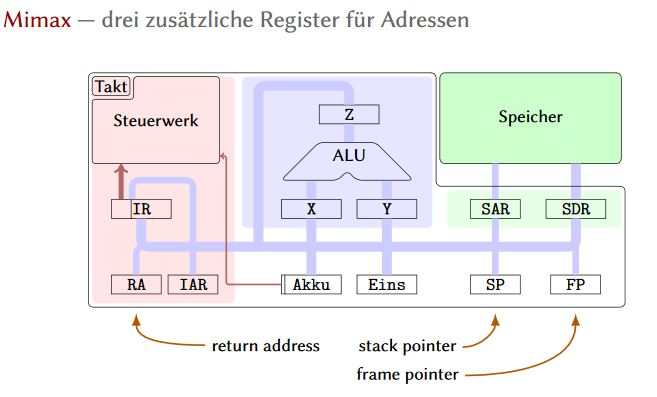
\includegraphics[width=\textwidth]{../topics/mimax/mimax_structure.jpg} 
\end{frame}

\begin{frame}{Neue Befehle}
	\begin{block}{CALL adr}
			\begin{itemize}
				\item ähnlich wie \emph{JMP} adr
				\item zusätzlich wird Inhalt vom IAR ins RA geschrieben
			\end{itemize}
		\end{block}
		
		\begin{block}{RET}
			\begin{itemize}
				\item ähnlich wie \emph{JMP} adr
				\item zusätzlich wird Inhalt vom RA ins IAR geschrieben
			\end{itemize}			
		\end{block}
	\emph{CALL adr} ruft also unsere Subroutine auf und mit \emph{RET} kehren wir von der Subroutine zurück zum Hauptprogramm
\end{frame}

\begin{frame}{Aufgabe}

	\begin{columns}
		\begin{column}{.4\textwidth}
			
			\begin{exampleblock}{Aufgabe}
				Schreibe ein Programm, das eine an Adresse $a$ gegebene Zahl mittels einer Subroutine negiert und danach wieder in $a$ speichert. Die Adresse $R$ sei zum Zwischenspeichern frei verfügbar.
			\end{exampleblock}
		\end{column}
	
		\begin{column}{.6\textwidth}
			\small \begin{tabular}{|l|l|}
			\toprule
				% Zugriffsoperationen
				LDC $c$ & $c \rightarrow Akku$ \\
				LDV $a$ & $M(a) \rightarrow Akku$ \\
				STV $a$ & $M(a) \leftarrow Akku$ \\
				LDIV $a$ & $M(M(a)) \rightarrow Akku$ \\
				STIV $a$ &$M(M(a)) \leftarrow Akku$ \\
				\midrule
				% Rechenoperationen
				ADD $a$ & $Akku + M(a) \rightarrow Akku$ \\
				AND $a$ & $Akku \ AND \ M(a) \rightarrow Akku$ \\
				OR $a$ & $Akku \ OR \ M(a) \rightarrow Akku$\\
				XOR $a$ & $Akku \ XOR \ M(a) \rightarrow Akku$\\
				NOT & Einskomplement von $Akku \rightarrow Akku$\\
				%RAR & rotiert $Akku$ um 1 nach rechts $\rightarrow Akku$\\
				\midrule
				% Vergleichsoperationen
				%EQL $a$ & $Akku \leftarrow \begin{cases}
											%-1 & \text{, falls } Akku = M(a) \\
											%0 & \text{, sonst} 
											%\end{cases}$\\
				%\midrule
				% Sprünge
				%JMP $a$ & fahre fort mit Befehl an der Adresse $a$\\
				%JMN $a$ & falls $Akku < 0$: JMP $a$\\
				CALL $a$ & rufe Subroutine an $M(a)$ auf\\
				RET & beende Subroutine und kehre zurück\\
				HALT & stoppt die Mima\\
			\bottomrule	
		\end{tabular}
		\end{column}
	\end{columns}
\end{frame}

\begin{frame}
	\begin{block}{Lösung}
		\emph{main}:LDV $a$\\
		CALL neg\\	
		HALT\\
		\emph{neg}:NOT\\
		STV $R$\\
		LDC 1\\
		ADD $R$\\
		STV $a$\\
		RET
	\end{block}
\end{frame}

\begin{frame}{Schnittstelle Stack}
	\begin{block}{Def.: Stack}
		\begin{itemize}
		\item Stapel von (Speicher-)Elementen
		\item Operationen: \begin{itemize}
			\item $push(e)$: Element $e$ oben auf den Stapel legen
			\item $pop()$: oberstes Element vom Stapel nehmen
			\item $top()$: oberstes Element anschauen
			%\item ($peek(k)$: Element an oberster $-k$ Stelle anschauen)
		\end{itemize}
	\end{itemize}
	\end{block}
\end{frame}

%\newcommand{\spmark}[1]{\colorbox{red!70}{#1}}
\begin{frame}{Stack im Speicher}
	\begin{itemize}
		\item Stackpointer (SP): Adresse der nächsten freien Stelle
		\item $push(e)$: \begin{enumerate}
			\item speichere $e$ an Adresse, auf die SP zeigt
			\item erhöhe SP um 1
		\end{enumerate}
	\end{itemize}

	\bigskip
	\textbf{Beispiel:}
	\begin{columns}
		\begin{column}{.3\textwidth}
			\centering \begin{tabular}{cc|c}
				& Adr & Val \\
				\cline{2-3}
				& $0$ & $v_0$ \\
				& \vdots & \vdots \\
				SP $\rightarrow$ & $a$ & \\
				& $a + 1$ &  \\
				& $a + 2$ &  \\
				& \vdots & \vdots 
			\end{tabular}
		\end{column}
	
		\begin{column}{.3\textwidth}
			\centering \begin{tabular}{cc|c}
				& Adr & Val \\
				\cline{2-3}
				& $0$ & $v_0$ \\
				& \vdots & \vdots \\
				& $a$ & $e$\\
				SP $\rightarrow$ & $a + 1$ &  \\
				& $a + 2$ &  \\
				& \vdots & \vdots 
			\end{tabular}
		\end{column}
	\end{columns}
\end{frame}

\begin{frame}{Stack im Speicher}
	\begin{itemize}
		\item Stackpointer (SP): Adresse der nächsten freien Stelle
		\item $top()$: \begin{enumerate}
			\item gib Element an Adresse SP$-1$ aus
		\end{enumerate}
	\end{itemize}

	\bigskip
	\textbf{Beispiel:}
	\begin{columns}	
		\begin{column}{.3\textwidth}
			\centering \begin{tabular}{cc|c}
				& Adr & Val \\
				\cline{2-3}
				& $0$ & $v_0$ \\
				& \vdots & \vdots \\
				& $a$ & $e$\\
				SP $\rightarrow$ & $a + 1$ &  \\
				& $a + 2$ &  \\
				& \vdots & \vdots 
			\end{tabular}
		\end{column}
		\begin{column}{.3\textwidth}
			\centering \begin{tabular}{cc|c}
				& Adr & Val \\
				\cline{2-3}
				& $0$ & $v_0$ \\
				& \vdots & \vdots \\
				& $a$ & $e$\\
				SP $\rightarrow$ & $a + 1$ &  \\
				& $a + 2$ &  \\
				& \vdots & \vdots 
			\end{tabular}
		\end{column}
	\end{columns}
\end{frame}

\begin{frame}{Stack im Speicher}
	\begin{itemize}
		\item Stackpointer (SP): Adresse der nächsten freien Stelle
		\item $pop()$: \begin{enumerate}
			\item verringere SP um 1 (Element an neuem SP zählt nicht mehr als Teil des Stack)
		\end{enumerate}
	\end{itemize}

	\bigskip
	\textbf{Beispiel:}
	\begin{columns}	
		\begin{column}{.3\textwidth}
			\centering \begin{tabular}{cc|c}
				& Adr & Val \\
				\cline{2-3}
				& $0$ & $v_0$ \\
				& \vdots & \vdots \\
				& $a$ & $e$\\
				SP $\rightarrow$ & $a + 1$ &  \\
				& $a + 2$ &  \\
				& \vdots & \vdots 
			\end{tabular}
		\end{column}
		\begin{column}{.3\textwidth}
			\centering \begin{tabular}{cc|c}
				& Adr & Val \\
				\cline{2-3}
				& $0$ & $v_0$ \\
				& \vdots & \vdots \\
				SP $\rightarrow$ & $a$ & $e$\\
				& $a + 1$ &  \\
				& $a + 2$ &  \\
				& \vdots & \vdots 
			\end{tabular}
		\end{column}
	\end{columns}
\end{frame}

\begin{frame}{Neue Befehle MIMAX}

\begin{tabular}{|l|l|}
			\toprule
				% Zugriffsoperationen
				LDSP/LDFP/LDRA & $SP/FP/RA \rightarrow Akku$ \\
				STSP/STFP/STRA & $SP/FP/RA \leftarrow Akku$ \\
				LDVR $disp(a)$ & $M(a+disp) \rightarrow Akku$ \\
				STVR $disp(a)$ & $M(a+disp) \leftarrow Akku$ \\
				\midrule
				% Rechenoperationen
				ADC $c$ & $Akku + c \rightarrow Akku$ (auch neg. Konstanten nach VL!)\\
				%RAR & rotiert $Akku$ um 1 nach rechts $\rightarrow Akku$\\
				\midrule
				% Vergleichsoperationen
				%EQL $a$ & $Akku \leftarrow \begin{cases}
											%-1 & \text{, falls } Akku = M(a) \\
											%0 & \text{, sonst} 
											%\end{cases}$\\
				%\midrule
				% Sprünge
				%JMP $a$ & fahre fort mit Befehl an der Adresse $a$\\
				%JMN $a$ & falls $Akku < 0$: JMP $a$\\
				CALL $a$ & rufe Subroutine an $M(a)$ auf\\
				RET & beende Subroutine und kehre zurück\\
			\bottomrule	
		\end{tabular}

\bigskip

$c$: Konstante \\
$a$: Adresse \\
$M(a)$: Wert an Adresse $a$
	
\end{frame}

% \begin{frame}{SP und FP}
% 	\begin{block}{stack pointer}
% 		zeigt auf Stelle an die \emph{push} den nächsten Wert legen würde\\
% 		\emph{LDVR disp(SP)} holt oberstes Speicherelement in Akku\\
% 		\emph{STVR disp(SP)} speichert Akkuinhalt als oberstes Stackelement	
% 	\end{block}
% 	\begin{block}{frame pointer}
% 			funktioniert ähnlich wie SP, genaueres in anderen Vorlesungen
% 	\end{block}
% \end{frame}

% \begin{frame}
% 	Für Beispiele mit der pointer-Magie schaut euch am besten die Vorlesungsfolien an!
% \end{frame}
